\section{Architecture of the code}
\begin{figure}[h!]
\centering
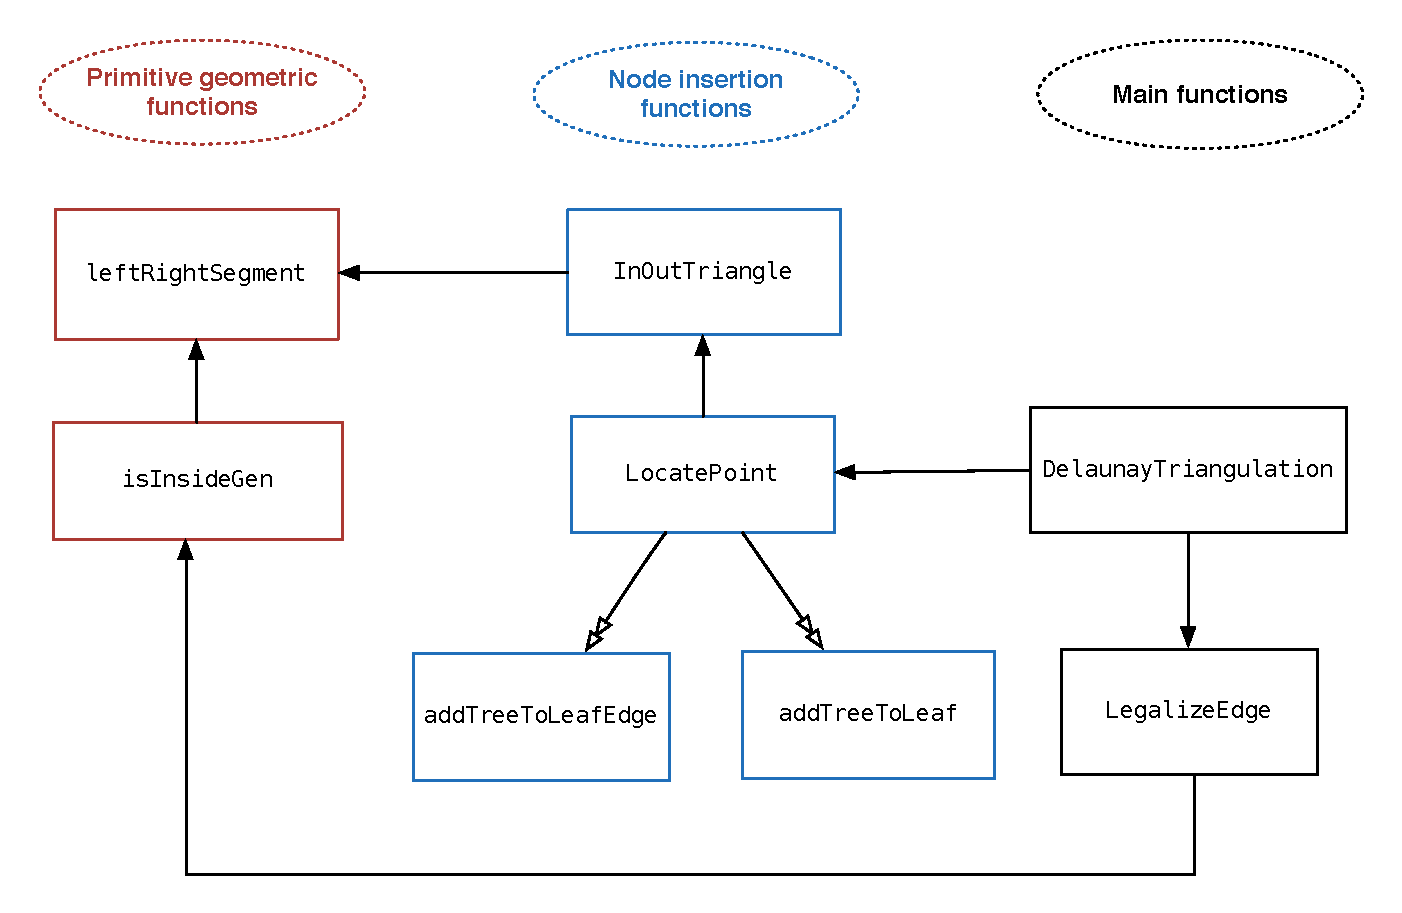
\includegraphics[width=0.8\textwidth]{images/Prog.eps}
\caption{Main architecture of the code. The simple arrows mean "use this function" and the double arrows mean "have as consequences".}
\label{fig:progArchitecture}
\end{figure}

Figure \ref{fig:progArchitecture} depicts the global architecture of our code. We have basically 4 types of functions : 
\begin{itemize}
\item the primitive \textbf{geometric functions} : 
\begin{enumerate}
\item \texttt{leftRightSegment} test whether a point lies on the right or on the left of a segment;
\item \texttt{isInsideGen} test whether a point lies inside or outside of a circle (it calls \texttt{leftRightSegment} because we need to have an oriented circle).
\end{enumerate}
It is important to notice that even if these functions seem trivial, they are the core of our code which determine the correctness of the code as we base all our processes on the answer of these functions. These are the only functions where we actually make computation (see section "Robustness" for more informations).
\item the \textbf{insertion functions} which performs 
\begin{enumerate}
\item the localisation step (the critical operation is \texttt{leftRightSegment} which is required to know in which triangle the point is);
\item the adding step : the point is added to the tree structure. 
\end{enumerate}
	Those functions are mainly manipulation of pointers and creation of  new structure's elements.
\item the \textbf{main functions} : 
\begin{enumerate}
\item \texttt{DelaunayTriangulation} which is the main function managing the Delaunay's triangulation;
\item \texttt{LegalizeEdge} which performs the pivot operation (the critical operation is \texttt{isInsideGen} which determine whether the pivot is performed or not).
\end{enumerate} 
\item the \textbf{maintenance functions} (useful but not interesting function, which is why they are not figured in figure \ref{fig:progArchitecture}) : 
\begin{enumerate}
\item the functions to create the structures (\texttt{meshPointCreate}, \texttt{meshEdgeCreate}...).
\item the stack functions useful to manipulate the stack (\texttt{DeleteStackElement}...)
\end{enumerate}
\item the graphical interface functions (in \texttt{glfem.c}).
\end{itemize}